\documentclass{article}
\usepackage[T1]{fontenc}
\usepackage{hyperref}
\usepackage{amsmath}
\usepackage[utf8]{inputenc}
\usepackage[polish]{babel}
\usepackage{graphicx}
\usepackage{amsfonts}
\usepackage{placeins}


\setlength{\textheight}{21cm}

\title{{\bf Zadanie nr 2 - Próbkowanie i kwantyzacja}\linebreak
Cyfrowe Przetwarzanie Sygnałów}
\author{Dominik Gałkowski, 247659 \and Jan Śladowski, 247806}
\date{29.04.2025}

\begin{document}
\clearpage\maketitle
\thispagestyle{empty}
\newpage
\setcounter{page}{1}
\section{Cel zadania}

Celem zadania jest zapoznanie się z praktycznymi zagadnieniami związanymi z konwersją sygnałów z postaci analogowej na cyfrową (A/C) oraz z cyfrowej na analogową (C/A), a także zaimplementowanie w programie z pierwszego zadania procesu konwersji analogowo-cyfrowej, obejmującego próbkowanie i kwantyzację, oraz procesu konwersji cyfrowo-analogowej.

\section{Wstęp teoretyczny}

Na podstawie instrukcji [1] do programu z zadania
pierwszego zostały dodane funkcjonalności do procesu konwersji analogowo-cyfrowej (A/C)
i cyfrowo-analogowej (C/A) sygnałów. Warto zaznaczyć, że zostały wykonane wszystkie
dostępne warianty z instrukcji do zadania i zostały one przedstawione poniżej:

\begin{itemize}
    \item {Konwersja A/C - próbkowanie}
    \begin{itemize}
        \item (S1) Próbkowanie równomierne
    \end{itemize}

    \item {Konwersja A/C - kwantyzacja}
    \begin{itemize}
        \item (Q1) Kwantyzacja równomierna z obcięciem
        \item (Q2) Kwantyzacja równomierna z zaokrąglaniem
    \end{itemize}

    \item {Konwersja C/A - rekonstrukcja sygnału}
    \begin{itemize}
        \item (R1) Ekstrapolacja zerowego rzędu
        \item (R2) Interpolacja pierwszego rzędu
        \item (R3) Rekonstrukcja w oparciu o funkcję sinc
    \end{itemize}
\end{itemize}

Co więcej należało zaimplementować miary, które służą do oceny zrekonstrułowanego
sygnału z oryginalnym na podstawie porównania częstotliwości próbkowania i progu
kwantyzacji oraz wyboru metody interpolacji. Miary zostały przedstawione poniżej:
\begin{itemize}
    \item {
        (C1) Błąd średniokwadratowy (MSE):
    }
    \item {
        (C2) Stosunek sygnał - szum (SNR):
    }
    \item {
        (C3) Szczytowy stosunek sygnał - szum (PSNR):
    }
    \item {
        (C4) Maksymalna różnica (MD):
    }
    \item {
        Efektywna liczba bitów (ENOB)
    }
\end{itemize}

\section{Materiały i metody} {
    Pojedyńczy eksperyment składał się z kilku kroków. W przypadku badania jakości
    rekonstrukcji sygnału wykonywaliśmy generowanie sygnału, następnie jego próbkowanie,
    następnie jego rekonstrukcje i porównanie sygnału pierwotnego z uzyskanym po rekonstrukcji.
    Dla badania kwantyzacji kroki były analogiczne z tą różnicą, że krok rekonstrukcji był zastępowany przez
    kwantyzację. Kolorem zielonym został oznaczony sygnał pierwotny natomiast kolorem niebieskim
    sygnał po rekonstrukcji lub kwantyzacji zależnie od przeprowadzanego eksperymentu.\\
}

\section{Eksperymenty i wyniki}



%%%%%%%%%%%%%%%%%%%%%%%%%%%%%%%%%%%%%%%%%%%%%%%%%%%%%%%%%%%%%%%%%%%%%%%%%%%%%%%%%%%%%%%%%%%%%%%%%%%%%%%%%%%%%%%%%
% PODROZDZIA� PT. EKSPERYMENT NR 1 
%%%%%%%%%%%%%%%%%%%%%%%%%%%%%%%%%%%%%%%%%%%%%%%%%%%%%%%%%%%%%%%%%%%%%%%%%%%%%%%%%%%%%%%%%%%%%%%%%%%%%%%%%%%%%%%%%

\subsection{Eksperyment 1}
    Celem eksperymentu było zbadanie wpływu zależności między częstotliwością
    sygnału a częstotliwością próbkowania na jakość rekonstrukcji

    \subsubsection{Założenia}
    \begin{table}[h!]
        \centering
        \begin{tabular}{|c|c|c|c|c|}
            \hline
            Funkcja & Czas trwania & Okres & Amplituda & Czas początkowy \\ \hline
            Sinusoidalna & 5 & 1 & 1 & 0   \\ \hline
        \end{tabular}
        \caption{Parametry wejściowe}
    \end{table}
    
    \subsubsection{Eksperyment}

    \begin{table}[h!]
        \centering
        \vspace{0.2cm}
        \begin{tabular}{|c|c|c|c|c|c|c|c|}
            \hline\hline\\[-0.4cm]
            Nr & \shortstack{Częstotliwość\\ próbkowania} & \shortstack{Metoda\\ rekonstrukcji} & MSE & SNR & PSNR & MD & ENOB  \\
            \hline
            1 & 3 & Sinc (100) & 0.570 & -0.608 & 2.689 & 1.645 & -0.393 \\
            \hline
            2 & 5 & Sinc (100) & 0.233 & 3.374 & 6.544 & 1.096 & 0.268   \\
            \hline
            3 & 10 & Sinc (100) & 0.062 & 9.138 & 12.062 & 0.582 & 1.226   \\
            \hline
            4 & 3 & Zero\_order & 0.573 & -0.590 & 1.793 & 1.727 & -0.390  \\
            \hline
            5 & 5 & Zero\_order & 0.223 & 3.513 & 6.300 & 1.170 & 0.291   \\
            \hline
            6 & 10 & Zero\_order & 0.048 & 10.189 & 12.988 & 0.583 & 1.400   \\
            \hline
            7 & 3 & First\_order & 0.460 & -2.645 & 2.749 & 1.644 & -0.732   \\
            \hline
            8 & 5 & First\_order & 0.211 & 2.651 & 6.539 & 1.083 & 0.148   \\
            \hline
            9 & 10 & First\_order & 0.060 & 8.992 & 12.004 & 0.582 & 1.201   \\
            \hline
        \end{tabular}
        \caption{Wyniki eksperymentu}
    \end{table}
    \FloatBarrier

    \begin{figure}[h!]
        \centering
        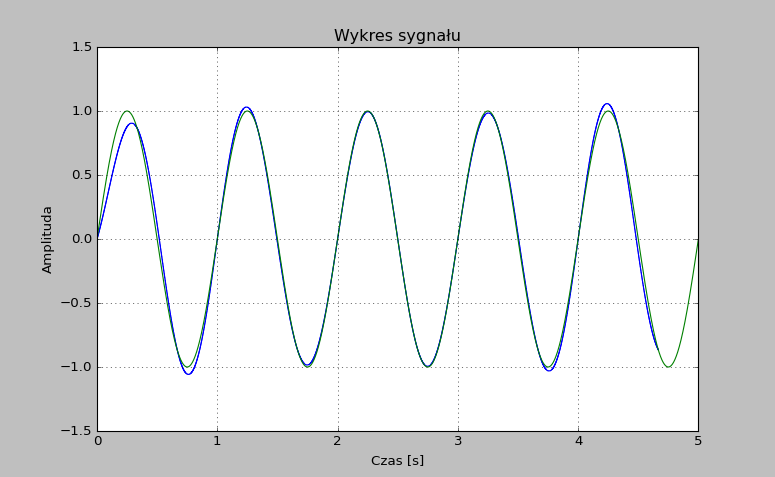
\includegraphics[width=0.8\textwidth]{img/1/sinc3.png}
        \caption{Wykres sygnałów przypadku nr 1}
    \end{figure}
    \FloatBarrier

    \begin{figure}[h!]
        \centering
        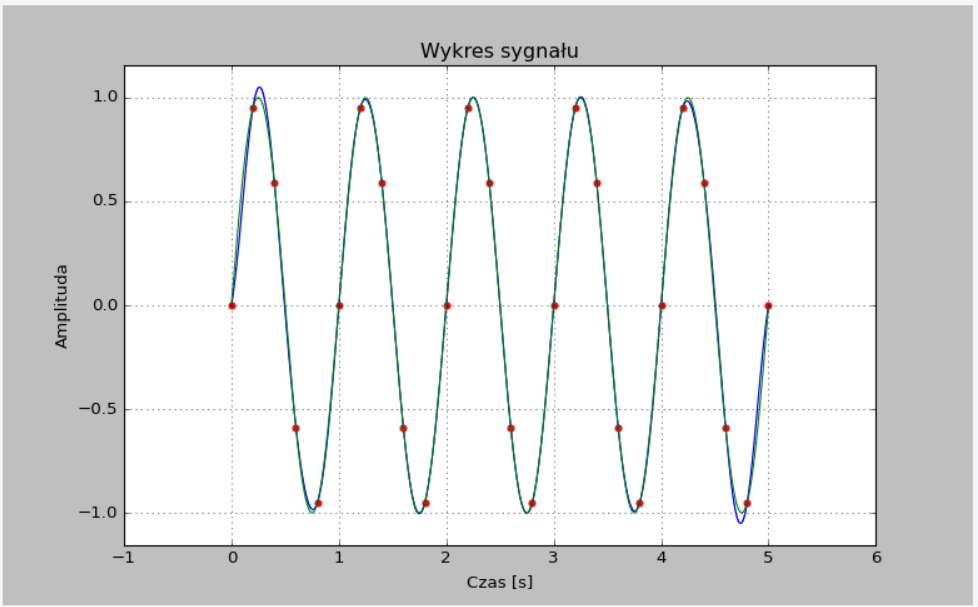
\includegraphics[width=0.8\textwidth]{img/1/sinc5.png}
        \caption{Wykres sygnałów przypadku nr 2}
    \end{figure}
    \FloatBarrier

    \begin{figure}[h!]
        \centering
        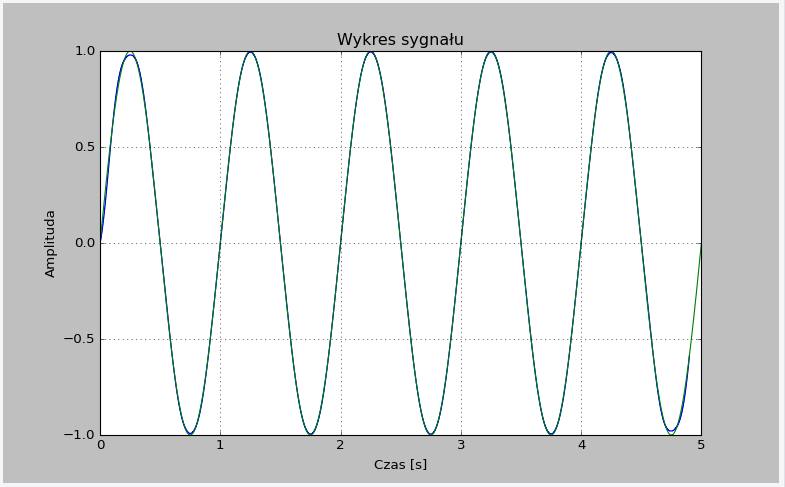
\includegraphics[width=0.8\textwidth]{img/1/sinc10.png}
        \caption{Wykres sygnałów przypadku nr 3}
    \end{figure}
    \FloatBarrier

    \begin{figure}[h!]
        \centering
        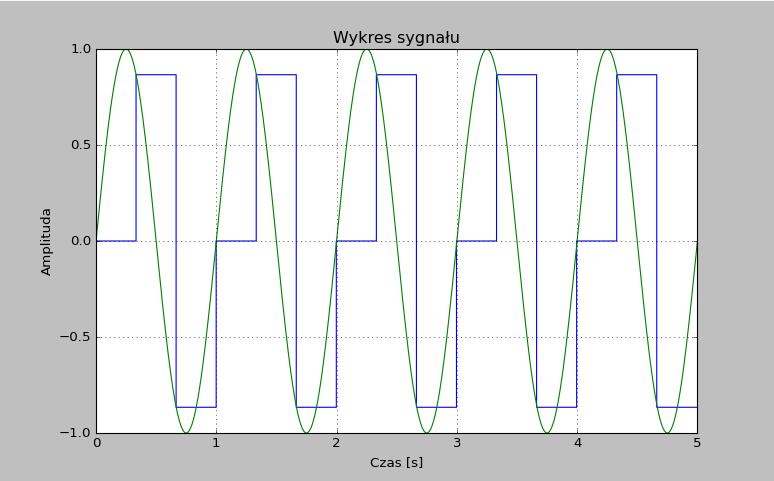
\includegraphics[width=0.8\textwidth]{img/1/zoh3.png}
        \caption{Wykres sygnałów przypadku nr 4}
    \end{figure}
    \FloatBarrier

    \begin{figure}[h!]
        \centering
        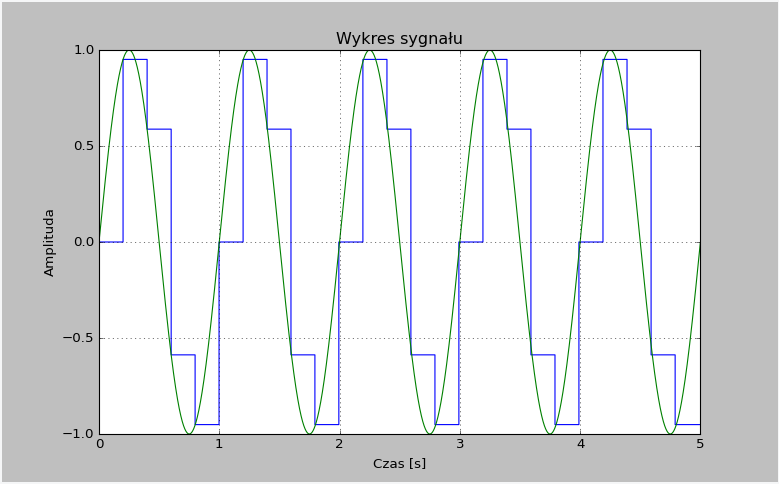
\includegraphics[width=0.8\textwidth]{img/1/zoh5.png}
        \caption{Wykres sygnałów przypadku nr 5}
    \end{figure}
    \FloatBarrier

    \begin{figure}[h!]
        \centering
        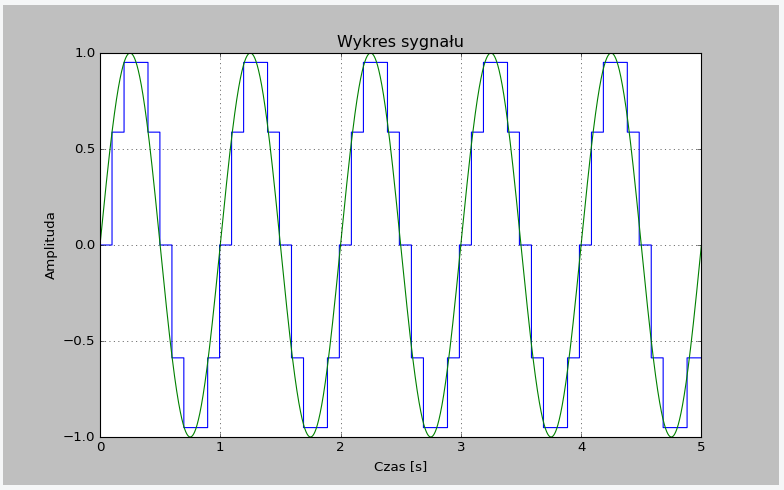
\includegraphics[width=0.8\textwidth]{img/1/zho10.png}
        \caption{Wykres sygnałów przypadku nr 6}
    \end{figure}
    \FloatBarrier

    \begin{figure}[h!]
        \centering
        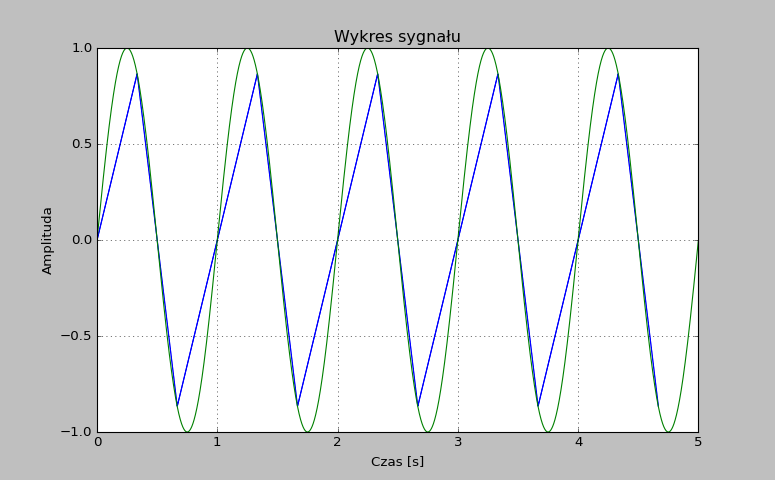
\includegraphics[width=0.8\textwidth]{img/1/foh3.png}
        \caption{Wykres sygnałów przypadku nr 7}
    \end{figure}
    \FloatBarrier

    \begin{figure}[h!]
        \centering
        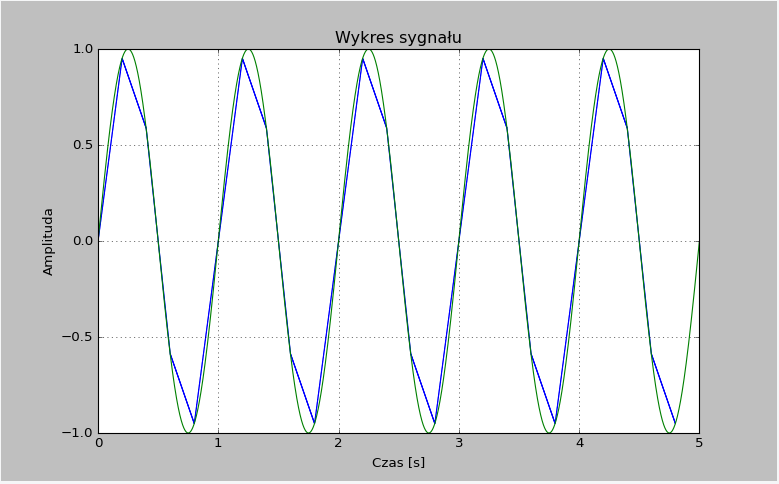
\includegraphics[width=0.8\textwidth]{img/1/foh5.png}
        \caption{Wykres sygnałów przypadku nr 8}
    \end{figure}
    \FloatBarrier

    \begin{figure}[h!]
        \centering
        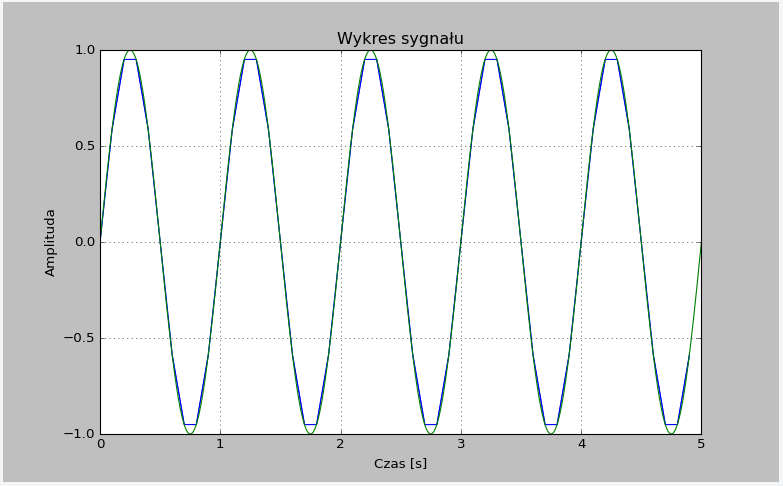
\includegraphics[width=0.8\textwidth]{img/1/foh10.png}
        \caption{Wykres sygnałów przypadku nr 9}
    \end{figure}
    \FloatBarrier

\subsection{Eksperyment 2}
    Celem eksperymentu było zbadanie wpływu rodzaju sygnału na jakość
    rekonstrukcji

    \subsubsection{Założenia}
    \begin{table}[h!]
        \centering
        \begin{tabular}{|c|c|c|c|c|c|}
            \hline
            \shortstack{Częstotliwość\\ próbkowania} & \shortstack{Czas\\ trwania} & Okres & Amplituda & \shortstack{Czas\\ początkowy} & \shortstack{Wspólczynnik\\ wypełnienia}   \\ \hline
            5 & 5 & 1 & 1 & 0 & 0.6  \\ \hline
        \end{tabular}
        \caption{Parametry wejściowe}
    \end{table}
    
    \subsubsection{Eksperyment}

    \begin{table}[h!]
        \centering
        \vspace{0.2cm}
        \begin{tabular}{|c|c|c|c|c|c|c|c|}
            \hline\hline\\[-0.4cm]
            Nr & Funkcja & \shortstack{Metoda\\ rekonstrukcji} & MSE & SNR & PSNR & MD & ENOB  \\
            \hline
            1 & Sinusoidalna & Sinc (100) & 0.233 & 3.374 & 6.544 & 1.096 & 0.268  \\
            \hline
            2 & Prostokątny & Sinc (100) & 0.201 & 3.409 & 8.259 & 1.090 & 0.274   \\
            \hline
            3 & Trójkątny & Sinc (100) & 0.057 & 8.192 & 12.474 & 0.593 & 1.068   \\
            \hline
            4 & Sinusoidalna & Zero\_order & 0.223 & 3.513 & 6.300 & 1.170 & 0.291  \\
            \hline
            5 & Prostokątny & Zero\_order & 0.160 & 4.385 & 7.959 & 1.000 & 0.436   \\
            \hline
            6 & Trójkątny & Zero\_order & 0.051 & 8.530 & 12.958 & 0.497 & 1.125   \\
            \hline
            7 & Sinusoidalna & First\_order & 0.211 & 2.651 & 6.539 & 1.083 & 0.148    \\
            \hline
            8 & Prostokątny & First\_order & 0.172 & 3.385 & 7.645 & 1.000 & 0.270   \\
            \hline
            9 & Trójkątny & First\_order & 0.046 & 8.707 & 13.344 & 0.497 & 1.154   \\
            \hline
        \end{tabular}
        \caption{Wyniki eksperymentu}
    \end{table}
    \FloatBarrier

    \begin{figure}[h!]
        \centering
        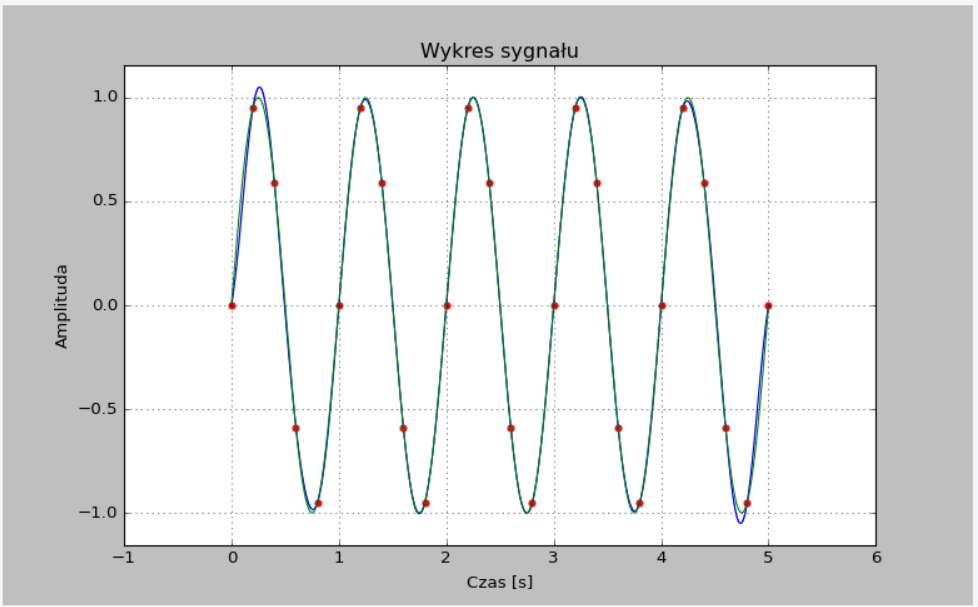
\includegraphics[width=0.8\textwidth]{img/1/sinc5.png}
        \caption{Wykres sygnałów przypadku nr 1}
    \end{figure}
    \FloatBarrier

    \begin{figure}[h!]
        \centering
        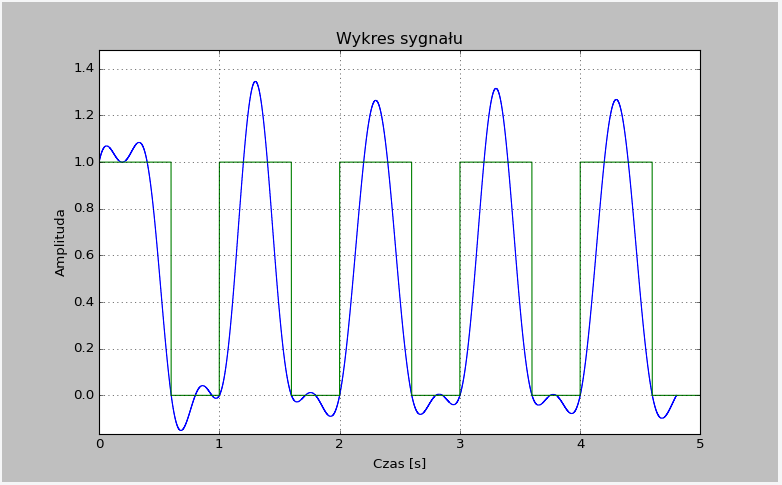
\includegraphics[width=0.8\textwidth]{img/1/sinc_rec.png}
        \caption{Wykres sygnałów przypadku nr 2}
    \end{figure}
    \FloatBarrier

    \begin{figure}[h!]
        \centering
        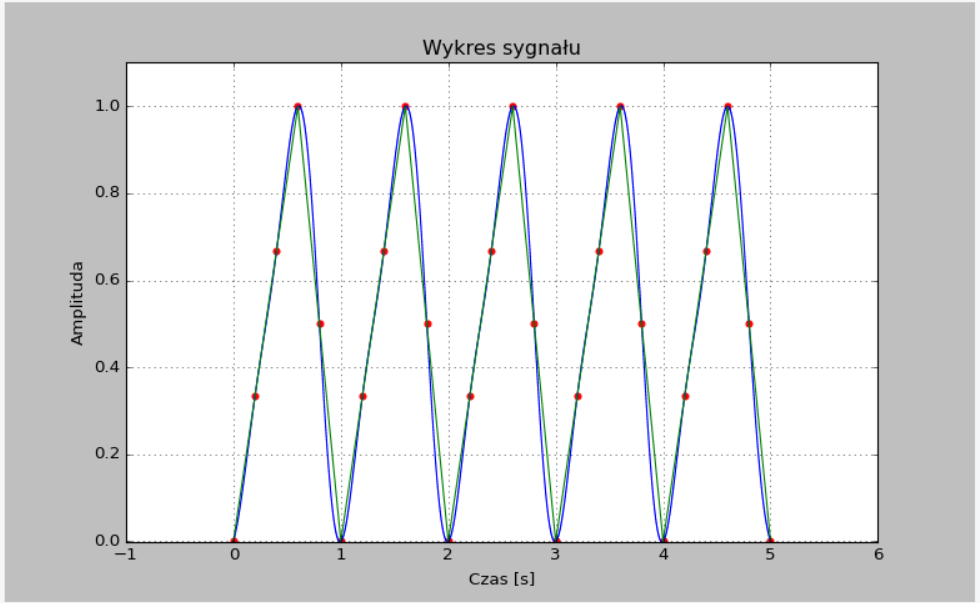
\includegraphics[width=0.8\textwidth]{img/1/sinc_tri.png}
        \caption{Wykres sygnałów przypadku nr 3}
    \end{figure}
    \FloatBarrier

    \begin{figure}[h!]
        \centering
        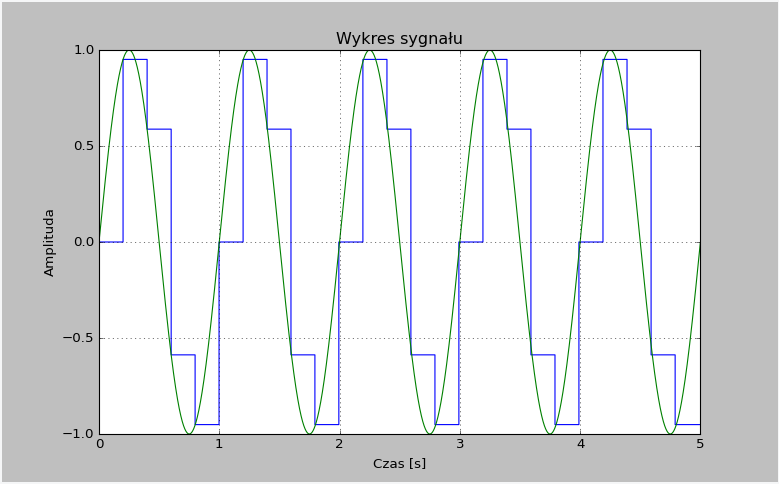
\includegraphics[width=0.8\textwidth]{img/1/zoh5.png}
        \caption{Wykres sygnałów przypadku nr 4}
    \end{figure}
    \FloatBarrier

    \begin{figure}[h!]
        \centering
        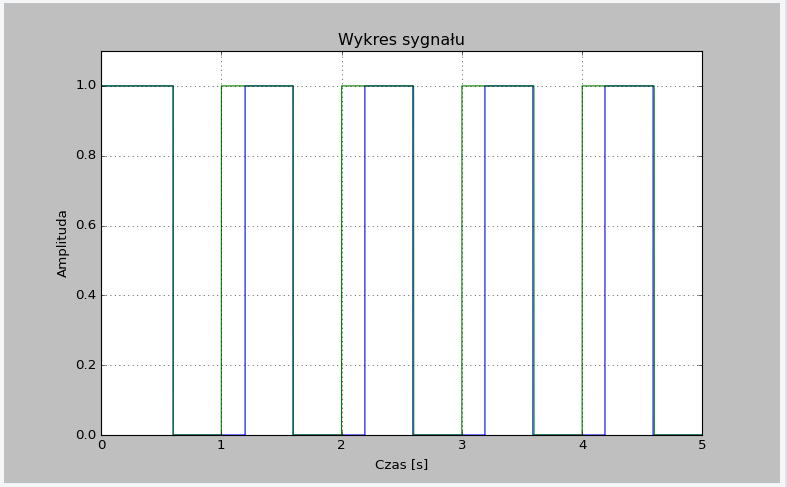
\includegraphics[width=0.8\textwidth]{img/1/zoh_rec.png}
        \caption{Wykres sygnałów przypadku nr 5}
    \end{figure}
    \FloatBarrier

    \begin{figure}[h!]
        \centering
        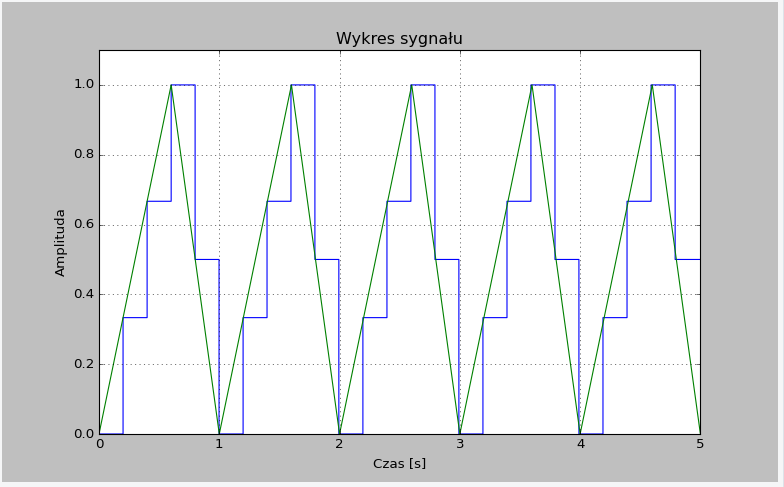
\includegraphics[width=0.8\textwidth]{img/1/zoh_tri.png}
        \caption{Wykres sygnałów przypadku nr 6}
    \end{figure}
    \FloatBarrier

    \begin{figure}[h!]
        \centering
        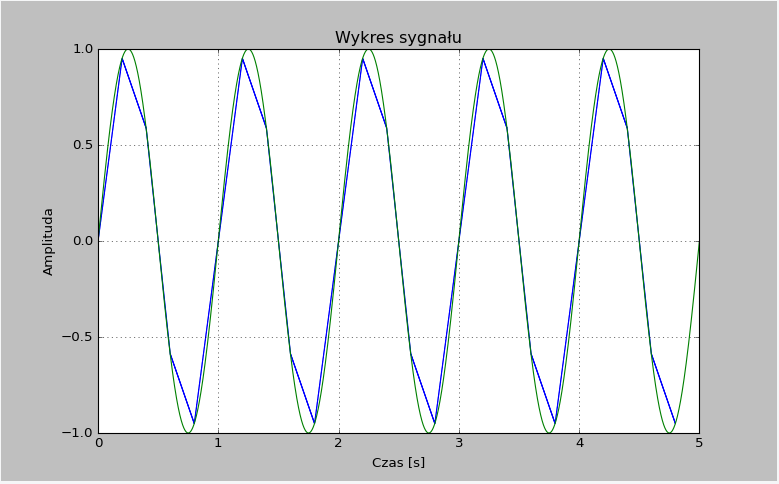
\includegraphics[width=0.8\textwidth]{img/1/foh5.png}
        \caption{Wykres sygnałów przypadku nr 7}
    \end{figure}
    \FloatBarrier

    \begin{figure}[h!]
        \centering
        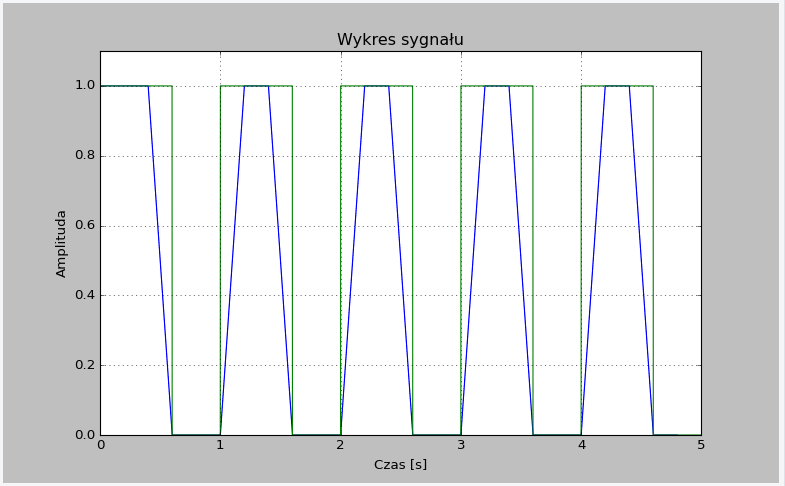
\includegraphics[width=0.8\textwidth]{img/1/foh_rec.png}
        \caption{Wykres sygnałów przypadku nr 8}
    \end{figure}
    \FloatBarrier

    \begin{figure}[h!]
        \centering
        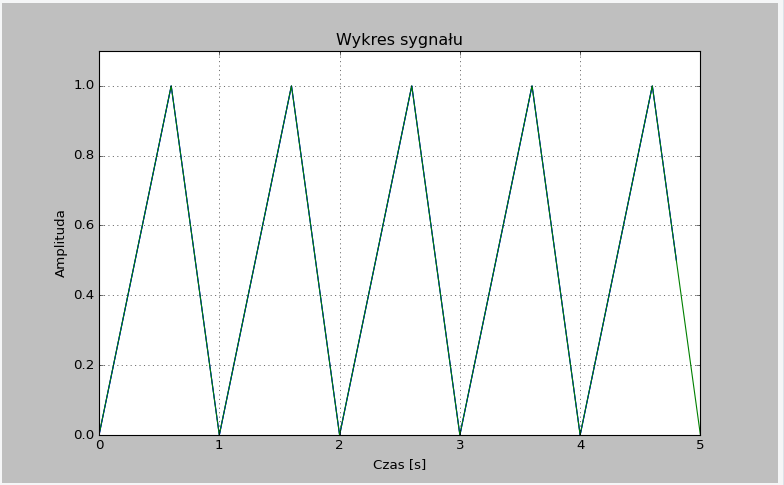
\includegraphics[width=0.8\textwidth]{img/1/foh_tri.png}
        \caption{Wykres sygnałów przypadku nr 9}
    \end{figure}
    \FloatBarrier

    \subsection{Eksperyment 3}
    Celem eksperymentu było zbadanie wpływu wartości N na jakość
    rekonstrukcji przy wykorzystaniu metody sinc

    \subsubsection{Założenia}
    \begin{table}[h!]
        \centering
        \begin{tabular}{|c|c|c|c|c|c|}
            \hline
            Funkcja & \shortstack{Częstotliwość\\ próbkowania} & \shortstack{Czas\\ trwania} & Okres & Amplituda & \shortstack{Czas\\ początkowy}  \\ \hline
            Sinusoidalna & 5 & 5 & 1 & 1 & 0  \\ \hline
        \end{tabular}
        \caption{Parametry wejściowe}
    \end{table}
    
    \subsubsection{Eksperyment}

    \begin{table}[h!]
        \centering
        \vspace{0.2cm}
        \begin{tabular}{|c|c|c|c|c|c|c|c|}
            \hline\hline\\[-0.4cm]
            Nr & N & \shortstack{Metoda\\ rekonstrukcji} & MSE & SNR & PSNR & MD & ENOB  \\
            \hline
            1 & 1 & Sinc & 0.453 & -3.176 & 3.220 & 1.308 & -0.820 \\
            \hline
            2 & 2 & Sinc & 0.329 & -1.717 & 4.610 & 1.106 & -0.578    \\
            \hline
            3 & 3 & Sinc & 0.191 & 4.792 & 7.331 & 1.082 & 0.504    \\
            \hline
            4 & 4 & Sinc & 0.173 & 4.674 & 8.150 & 1.082 & 0.484  \\
            \hline
            5 & 5 & Sinc & 0.237 & 3.435 & 6.387 & 1.085 & 0.278    \\
            \hline
            6 & 10 & Sinc & 0.214 & 3.674 & 6.976 & 1.105 & 0.318   \\
            \hline
            7 & 25 & Sinc & 0.233 & 3.374 & 6.544 & 1.096 & 0.268   \\
            \hline
            8 & 50 & Sinc & 0.233 & 3.374 & 6.544 & 1.096 & 0.268   \\
            \hline
            9 & 100 & Sinc & 0.233 & 3.374 & 6.544 & 1.096 & 0.268  \\
            \hline
        \end{tabular}
        \caption{Wyniki eksperymentu}
    \end{table}
    \FloatBarrier

    \begin{figure}[h!]
        \centering
        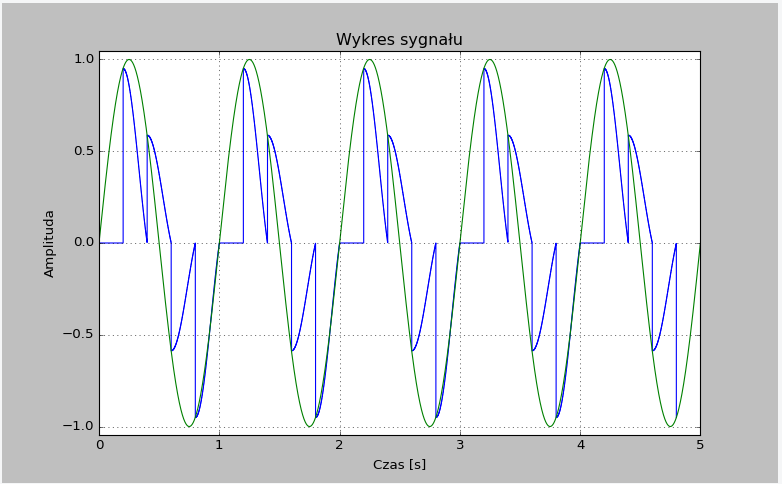
\includegraphics[width=0.8\textwidth]{img/1/sinc1.png}
        \caption{Wykres sygnałów przypadku nr 1}
    \end{figure}
    \FloatBarrier

    \begin{figure}[h!]
        \centering
        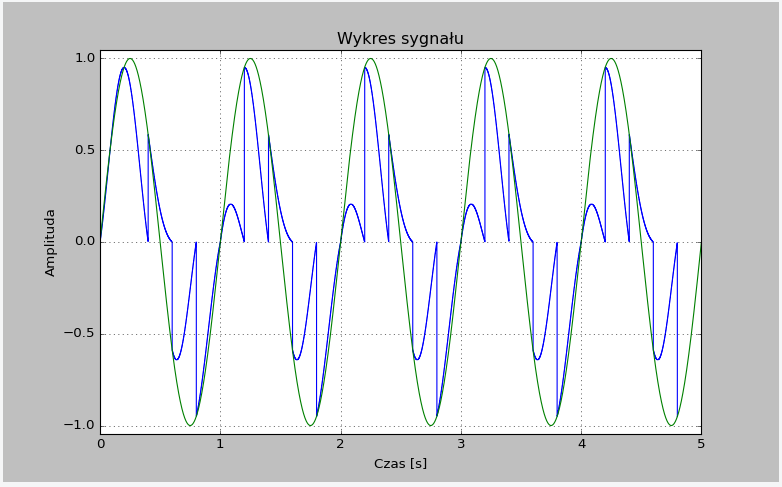
\includegraphics[width=0.8\textwidth]{img/1/sinc2.png}
        \caption{Wykres sygnałów przypadku nr 2}
    \end{figure}
    \FloatBarrier

    \begin{figure}[h!]
        \centering
        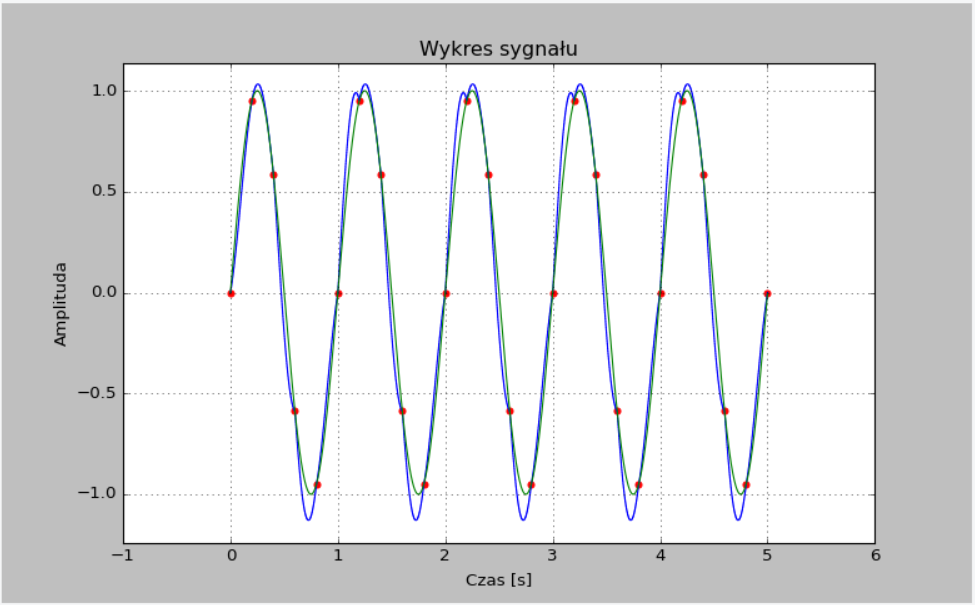
\includegraphics[width=0.8\textwidth]{img/1/sinc_3.png}
        \caption{Wykres sygnałów przypadku nr 3}
    \end{figure}
    \FloatBarrier

    \begin{figure}[h!]
        \centering
        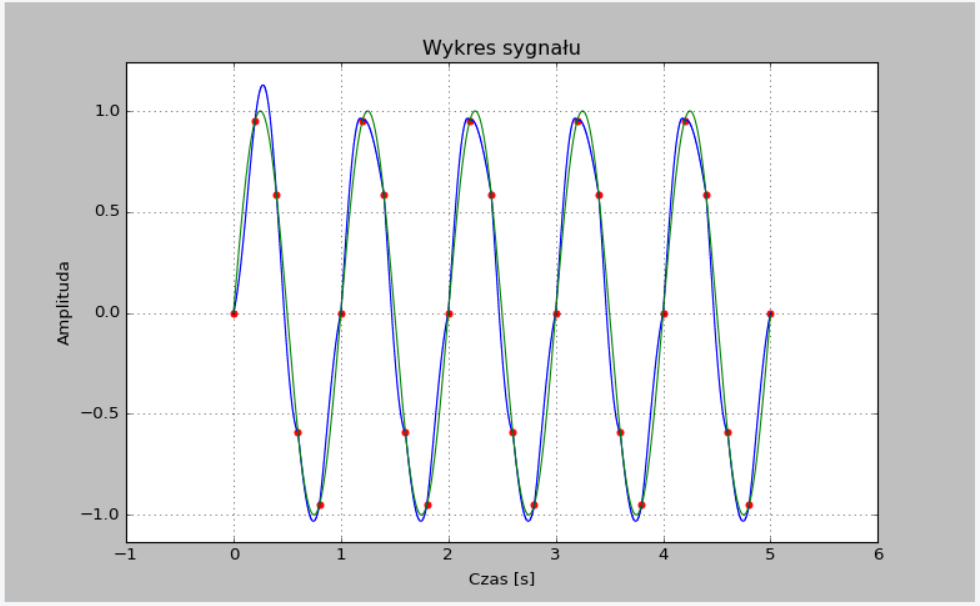
\includegraphics[width=0.8\textwidth]{img/1/sinc4.png}
        \caption{Wykres sygnałów przypadku nr 4}
    \end{figure}
    \FloatBarrier

    \begin{figure}[h!]
        \centering
        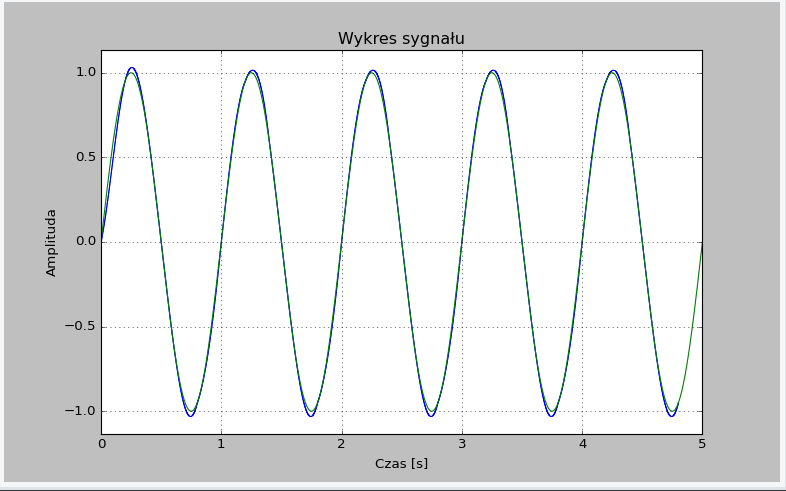
\includegraphics[width=0.8\textwidth]{img/1/sinc_5.png}
        \caption{Wykres sygnałów przypadku nr 5}
    \end{figure}
    \FloatBarrier

    \begin{figure}[h!]
        \centering
        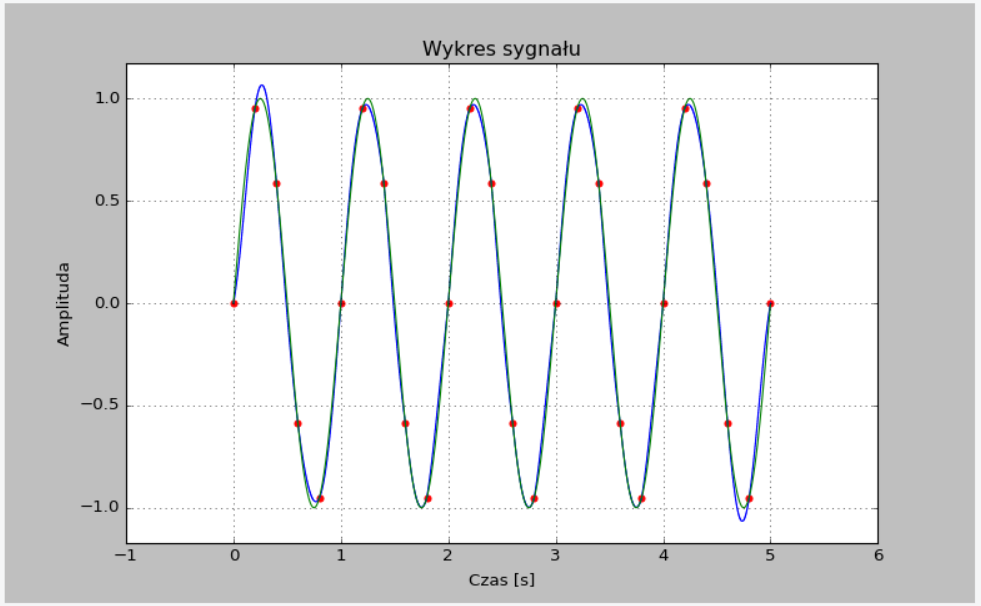
\includegraphics[width=0.8\textwidth]{img/1/sinc_10.png}
        \caption{Wykres sygnałów przypadku nr 6}
    \end{figure}
    \FloatBarrier

    \begin{figure}[h!]
        \centering
        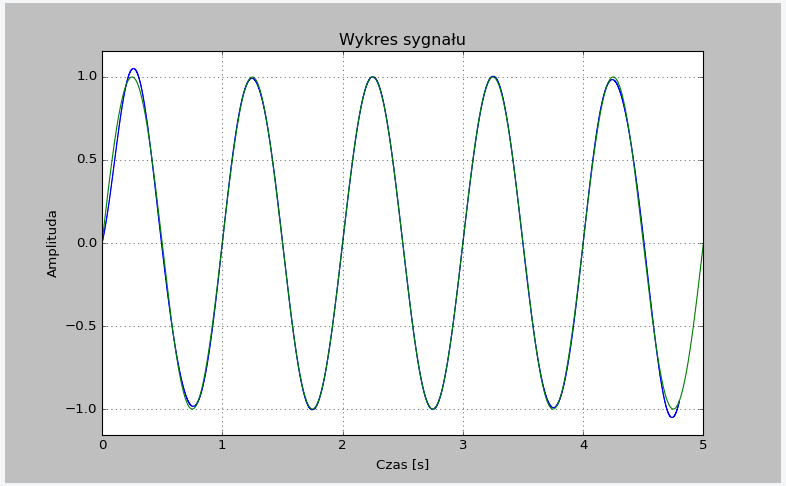
\includegraphics[width=0.8\textwidth]{img/1/sinc25.png}
        \caption{Wykres sygnałów przypadku nr 7}
    \end{figure}
    \FloatBarrier

    \begin{figure}[h!]
        \centering
        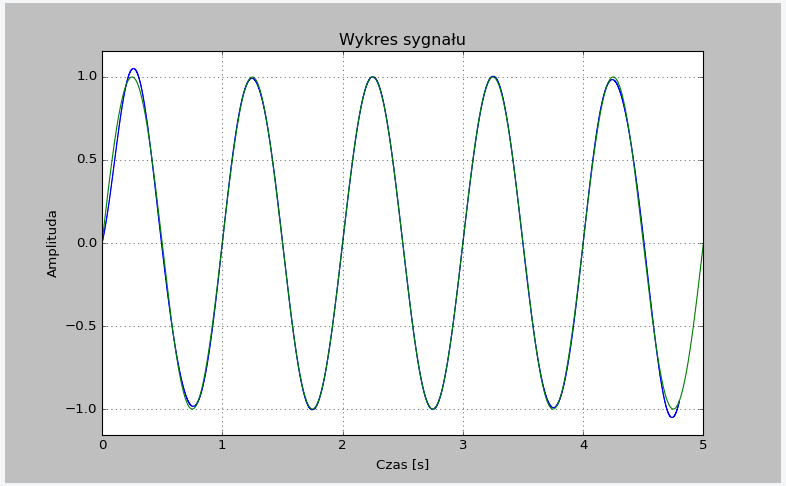
\includegraphics[width=0.8\textwidth]{img/1/sinc25.png}
        \caption{Wykres sygnałów przypadku nr 8}
    \end{figure}
    \FloatBarrier

    \begin{figure}[h!]
        \centering
        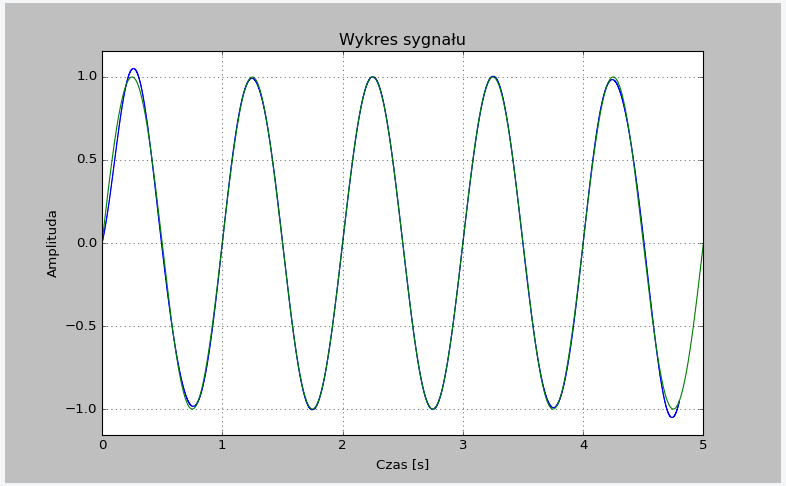
\includegraphics[width=0.8\textwidth]{img/1/sinc25.png}
        \caption{Wykres sygnałów przypadku nr 9}
    \end{figure}
    \FloatBarrier
    \subsection{Eksperyment 4}
    Celem eksperymentu było zbadanie wpływu liczby poziomów kwantyzacji sygnału na błąd
    kwantyzacji dla różnych sygnałów

    \subsubsection{Założenia}
    \begin{table}[h!]
        \centering
        \begin{tabular}{|c|c|c|c|c|c|}
            \hline
            \shortstack{Częstotliwość\\ próbkowania} & \shortstack{Czas\\ trwania} & Okres & Amplituda & \shortstack{Czas\\ początkowy} & \shortstack{Wspólczynnik\\ wypełnienia}   \\ \hline
            5 & 5 & 1 & 1 & 0 & 0.6  \\ \hline
        \end{tabular}
        \caption{Parametry wejściowe}
    \end{table}
    
    \subsubsection{Eksperyment}

    \begin{table}[h!]
        \centering
        \vspace{0.2cm}
        \begin{tabular}{|c|c|c|c|c|c|c|c|}
            \hline\hline\\[-0.4cm]
            Nr & Funkcja & Poziom & MSE & SNR & PSNR & MD & ENOB  \\
            \hline
            1 & Sinusoidalna & 2 & 0.234 & 5.878 & 6.096 & 0.951 & 0.684 \\
            \hline
            2 & Prostokątny & 2 & 0.000 & inf & inf & 0.000 & inf  \\
            \hline
            3 & Trójkątny & 2 & 0.090 & 7.604 & 10.444 & 0.500 & 0.971   \\
            \hline
            4 & Sinusoidalna & 5 & 0.005 & 19.529 & 22.757 & 0.112 & 2.952  \\
            \hline
            5 & Prostokątny & 5 & 0.000 & inf & inf & 0.000 & inf   \\
            \hline
            6 & Trójkątny & 5 & 0.003 & 20.846 & 25.563 & 0.083 & 3.170   \\
            \hline
            7 & Sinusoidalna & 10 & 0.004 & 21.156 & 24.164 & 0.106 & 3.222    \\
            \hline
            8 & Prostokątny & 10 & 0.000 & inf & inf & 0.000 & inf   \\
            \hline
            9 & Trójkątny & 10 & 0.001 & 24.109 & 28.573 & 0.056 & 3.713   \\
            \hline
        \end{tabular}
        \caption{Wyniki eksperymentu}
    \end{table}
    \FloatBarrier

    \begin{figure}[h!]
        \centering
        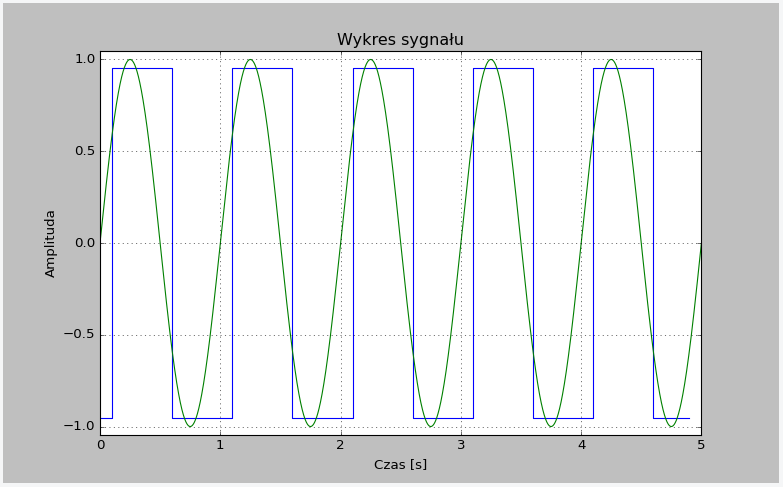
\includegraphics[width=0.8\textwidth]{img/1/quad_sin_2.png}
        \caption{Wykres sygnałów przypadku nr 1}
    \end{figure}
    \FloatBarrier

    \begin{figure}[h!]
        \centering
        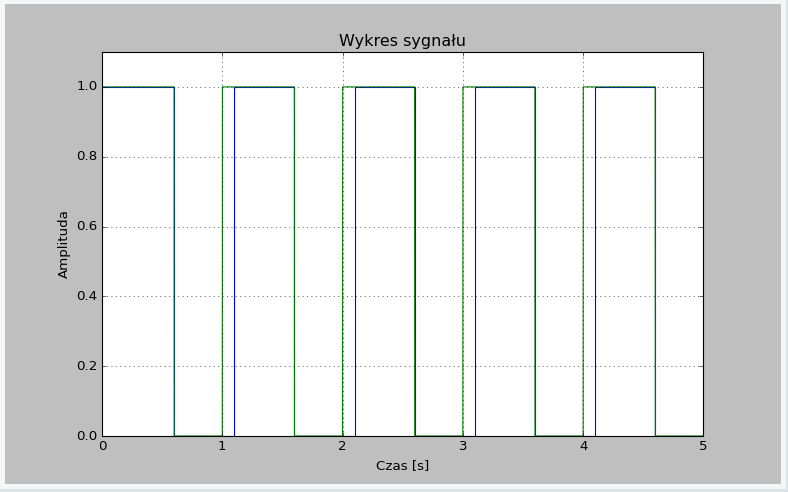
\includegraphics[width=0.8\textwidth]{img/1/quad_rect_2.png}
        \caption{Wykres sygnałów przypadku nr 2}
    \end{figure}
    \FloatBarrier

    \begin{figure}[h!]
        \centering
        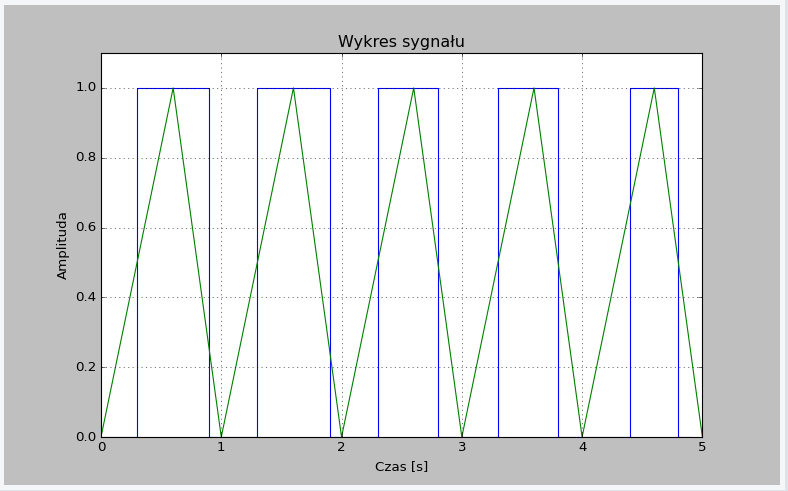
\includegraphics[width=0.8\textwidth]{img/1/quad_tri_2.png}
        \caption{Wykres sygnałów przypadku nr 3}
    \end{figure}
    \FloatBarrier

    \begin{figure}[h!]
        \centering
        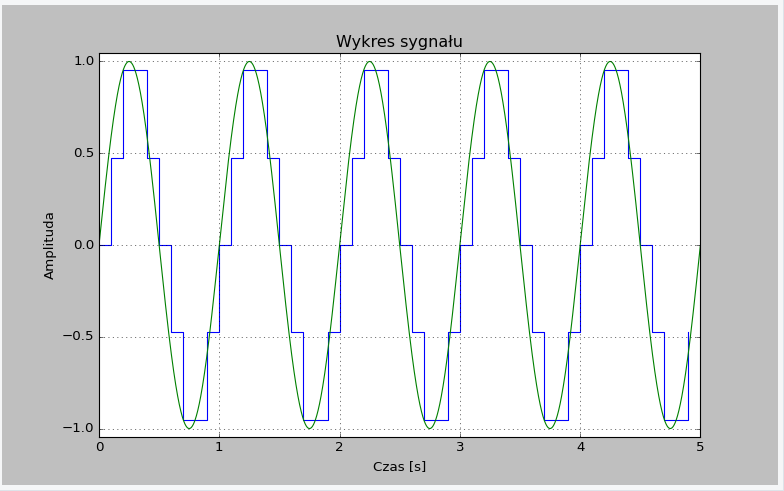
\includegraphics[width=0.8\textwidth]{img/1/quad_sin_5.png}
        \caption{Wykres sygnałów przypadku nr 4}
    \end{figure}
    \FloatBarrier

    \begin{figure}[h!]
        \centering
        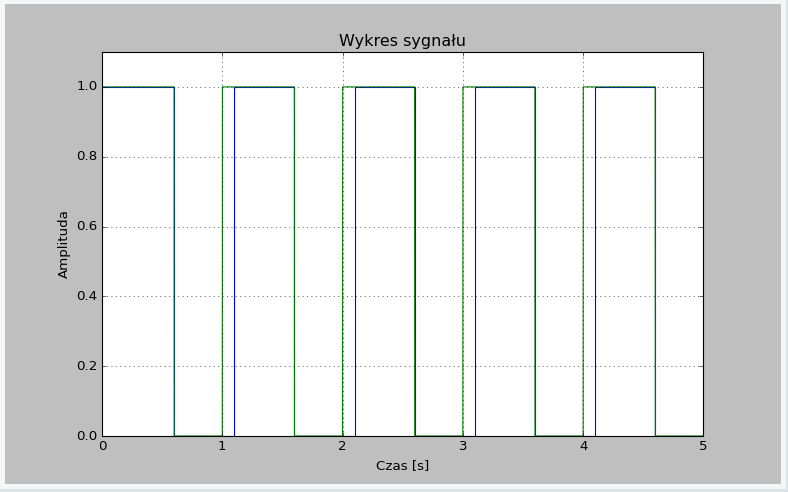
\includegraphics[width=0.8\textwidth]{img/1/quad_rect_2.png}
        \caption{Wykres sygnałów przypadku nr 5}
    \end{figure}
    \FloatBarrier

    \begin{figure}[h!]
        \centering
        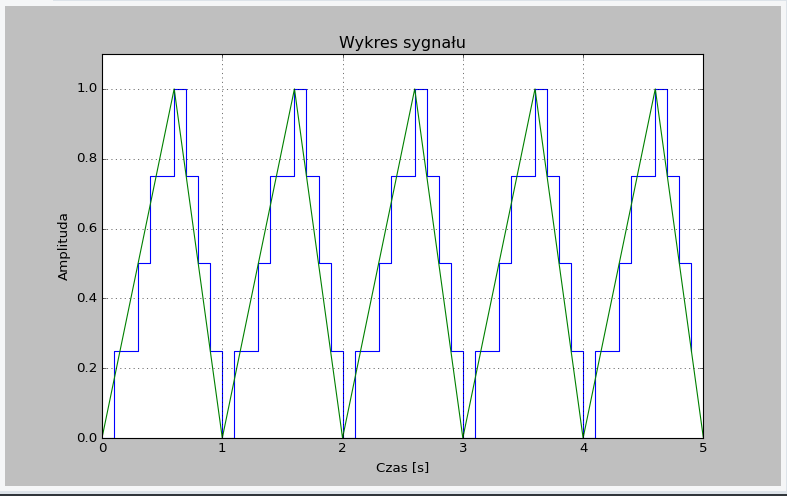
\includegraphics[width=0.8\textwidth]{img/1/quad_tri_5.png}
        \caption{Wykres sygnałów przypadku nr 6}
    \end{figure}
    \FloatBarrier

    \begin{figure}[h!]
        \centering
        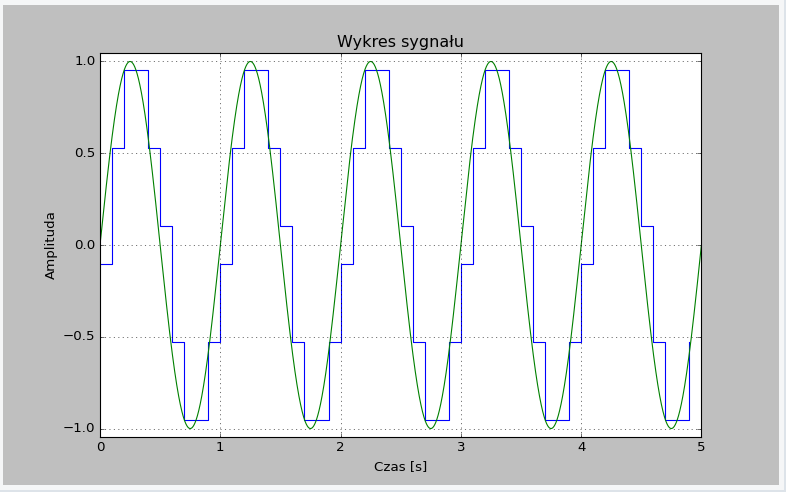
\includegraphics[width=0.8\textwidth]{img/1/quad_sin_10.png}
        \caption{Wykres sygnałów przypadku nr 7}
    \end{figure}
    \FloatBarrier

    \begin{figure}[h!]
        \centering
        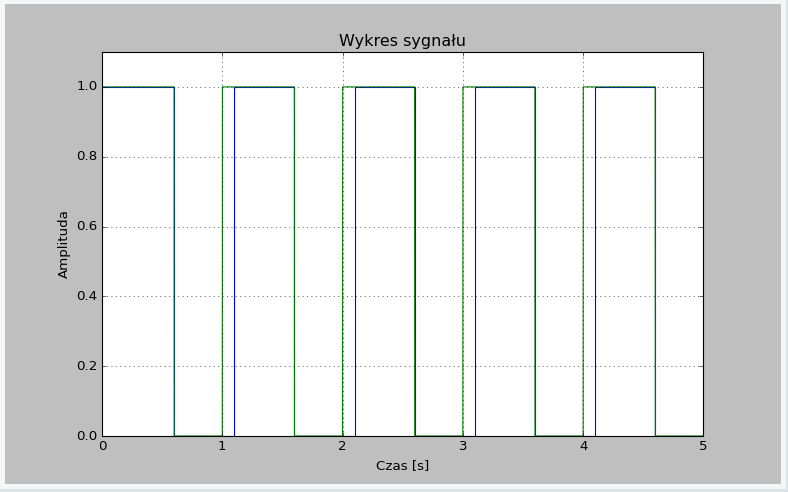
\includegraphics[width=0.8\textwidth]{img/1/quad_rect_2.png}
        \caption{Wykres sygnałów przypadku nr 8}
    \end{figure}
    \FloatBarrier

    \begin{figure}[h!]
        \centering
        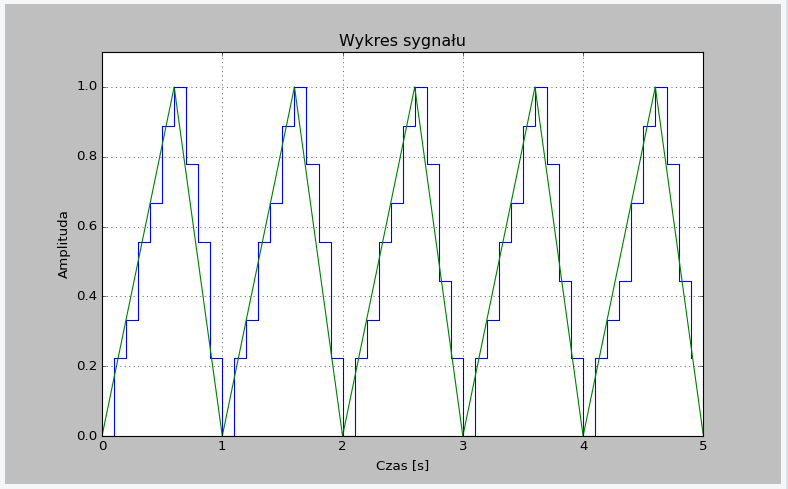
\includegraphics[width=0.8\textwidth]{img/1/quad_tri_10.png}
        \caption{Wykres sygnałów przypadku nr 9}
    \end{figure}
    \FloatBarrier
    \subsection{Eksperyment 5}
    Celem eksperymentu było zbadanie zjawiska aliasingu

    \subsubsection{Założenia}
    \begin{table}[h!]
        \centering
        \begin{tabular}{|c|c|c|c|c|c|}
            \hline
            Funkcja & \shortstack{Częstotliwość\\ próbkowania} & \shortstack{Czas\\ trwania} & \shortstack{Metoda\\ rekonstrukcji} & Amplituda & \shortstack{Czas\\ początkowy}  \\ \hline
            Sinusoidalna & 5 & 1 & Sinc (100) & 1 & 0  \\ \hline
        \end{tabular}
        \caption{Parametry wejściowe}
    \end{table}
    
    \subsubsection{Eksperyment}

    \begin{table}[h!]
        \centering
        \vspace{0.2cm}
        \begin{tabular}{|c|c|c|c|c|c|c|}
            \hline\hline\\[-0.4cm]
            Nr & Okres & MSE & SNR & PSNR & MD & ENOB  \\
            \hline
            1 & 0.143 & 0.887 & -3.312 & 0.428 & 1.980 & -0.843 \\
            \hline
            2 & 0.09 & 1.008 & -2.820 & 0.173 & 2.026 & -0.761  \\
            \hline
            3 & 0.083 & 0.887 & -3.370 & 0.534 & 1.926 & -0.852   \\
            \hline
        \end{tabular}
        \caption{Wyniki eksperymentu}
    \end{table}
    \FloatBarrier

    \begin{figure}[h!]
        \centering
        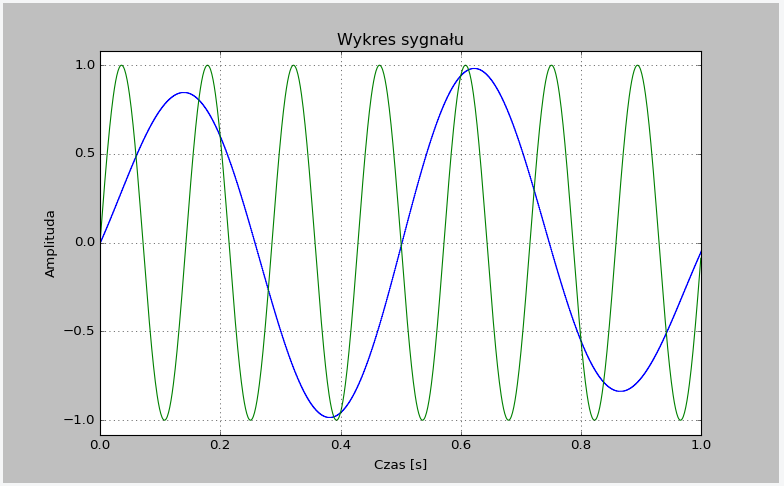
\includegraphics[width=0.8\textwidth]{img/1/anti_1.png}
        \caption{Wykres sygnałów przypadku nr 1}
    \end{figure}
    \FloatBarrier

    \begin{figure}[h!]
        \centering
        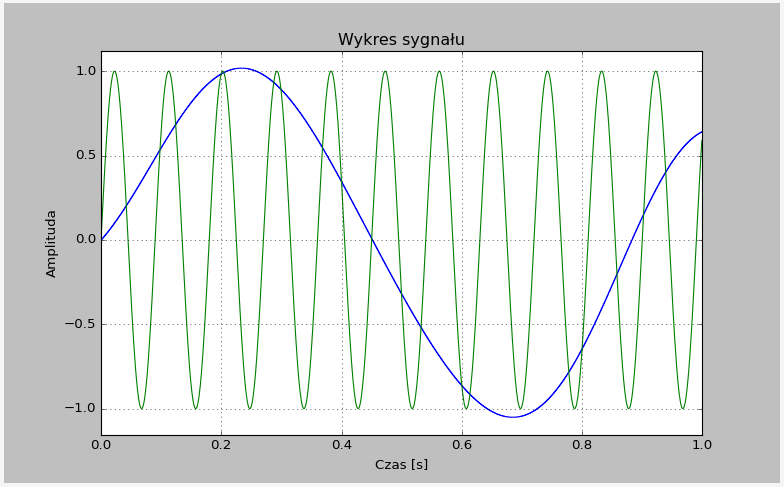
\includegraphics[width=0.8\textwidth]{img/1/anti_2.png}
        \caption{Wykres sygnałów przypadku nr 2}
    \end{figure}
    \FloatBarrier

    \begin{figure}[h!]
        \centering
        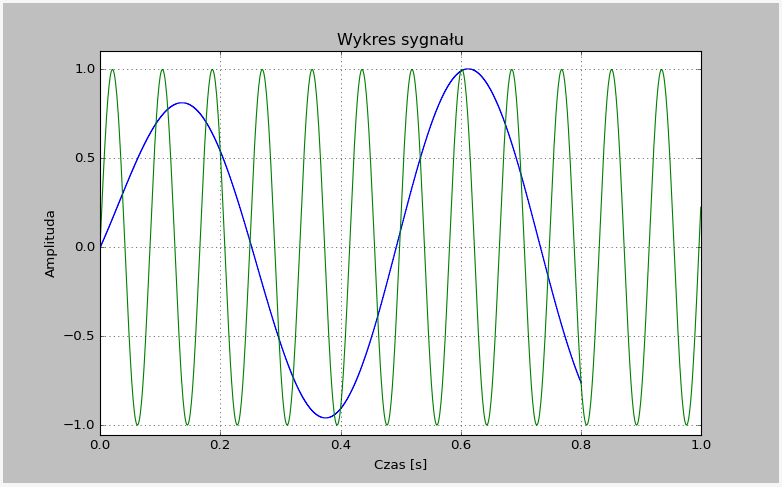
\includegraphics[width=0.8\textwidth]{img/1/anti_3.png}
        \caption{Wykres sygnałów przypadku nr 3}
    \end{figure}
    \FloatBarrier
\section{Dyskusja}
    \subsection{Eksperyment 1}
    W pierwszej serii eksperymentów przeanalizowano wpływ stosunku częstotliwości sygnału do częstotliwości 
    próbkowania na jakość rekonstrukcji sygnału przy zastosowaniu różnych metod. W badaniach rozważano 
    sygnały okresowe. We wszystkich przypadkach generowano sygnał sinusoidalny o okresie 
    $1,\mathrm{s}$ i czasie trwania $5,\mathrm{s}$. Zmiennymi w eksperymentach były metoda rekonstrukcji 
    oraz częstotliwość próbkowania, przy czym wartość częstotliwości próbkowania zawsze przekraczała 
    dwukrotność częstotliwości sygnału, co miało na celu eliminację zjawiska aliasingu (omówionego w dalszej 
    części opracowania).

    Analiza wyników eksperymentów 1–3, w których zastosowano rekonstrukcję opartą na funkcji \emph{sinc}, 
    wykazała jednoznaczną zależność: zwiększenie częstotliwości próbkowania skutkuje poprawą jakości odtworzonego 
    sygnału. Tendencję tę potwierdzają wartości wskaźników jakości: obserwuje się spadek wartości miar błędu, 
    takich jak MSE oraz MD, oraz wzrost wartości miar takich jak SNR i PSNR. Wzrast ze wzrostem częstoliowści
    próbkowania poprawiały się wyniki oraz powodowały poprawę rekonstrukcji, co było widoczne w analizie błędu
    średniokwadratowego. Wnioski te są również spójne z obserwacjami 
    jakościowymi wykresów — im bardziej częstotliwość próbkowania zbliżała się do minimalnej wymaganej wartości 
    (dwukrotność częstotliwości sygnału), tym bardziej zauważalne były zmiany jakości rekonstrukcji. 
    W dalszej kolejności zmiany te stawały się pomijalnie małe. Należy jednocześnie podkreślić, że na jakość 
    rekonstrukcji wpływ ma również liczba próbek oraz czas trwania analizowanego sygnału.

    Eksperymenty 4–6 obejmowały rekonstrukcję sygnału metodą ekstrapolacji zerowego rzędu. 
    W wyniku tej rekonstrukcji otrzymano funkcje złożone z odcinków o stałej wartości. 
    Zarówno analiza wartości miar jakości, jak i obserwacje wizualne wykazały, że metoda ta 
    charakteryzuje się znacznie niższą skutecznością niż rekonstrukcja oparta na funkcji \emph{sinc}.
    Choć wzrost częstotliwości próbkowania również powodował poprawę jakości odtworzonego sygnału, 
    skala tej poprawy była wyraźnie mniejsza w porównaniu do wyników uzyskanych metodą \emph{sinc}.

    Ostatnią analizowaną metodą rekonstrukcji była interpolacja pierwszego rzędu, w której do odtworzenia 
    sygnału wykorzystano funkcje liniowe. Wyniki eksperymentów wykazały, że metoda ta pozwala na uzyskanie 
    lepszej jakości rekonstrukcji niż ekstrapolacja zerowego rzędu, choć nadal pozostaje mniej efektywna niż 
    rekonstrukcja oparta na funkcji \emph{sinc}. Co istotne, wyniki uzyskane w eksperymencie 9 sugerują, że 
    przy odpowiednio dużej liczbie próbek interpolacja pierwszego rzędu może osiągnąć jakość porównywalną z 
    wynikami uzyskanymi metodą \emph{sinc}.
    
    \subsection{Eksperyment 2}
    W drugiej serii eksperymentów przeanalizowano wpływ typu sygnału na jakość jego rekonstrukcji przy 
    wykorzystaniu różnych metod odtwarzania. Badaniu poddano trzy rodzaje sygnałów okresowych: sinusoidalny, 
    prostokątny oraz trójkątny. Dla każdego z nich zastosowano wszystkie wcześniej opisane techniki 
    rekonstrukcji, co umożliwiło dokonanie porównania ich efektywności w zależności od charakterystyki 
    sygnału źródłowego.
    Eksperymenty oznaczone jako 1–3 koncentrowały się na zastosowaniu rekonstrukcji opartej na funkcji
    \emph{sinc}. Wyniki potwierdziły wysoką skuteczność tej metody w przypadku sygnału sinusoidalnego, 
    co jest zgodne z jej teoretycznymi właściwościami – funkcja \emph{sinc} stanowi bowiem idealny 
    interpolator w przypadku sygnałów będących kombinacją składowych harmonicznych. Z kolei dla sygnału
    prostokątnego metoda ta wykazała niską jakość odwzorowania, co wynika z obecności nieciągłości oraz
    dużej liczby wyższych harmonicznych, których precyzyjna rekonstrukcja wymaga znacznie większej liczby 
    próbek. Dla sygnału trójkątnego odnotowano nieco lepsze rezultaty niż w przypadku sygnału 
    prostokątnego, jednak jakość rekonstrukcji pozostawała zauważalnie niższa niż w przypadku sygnału 
    sinusoidalnego.
    Eksperyment 4 obejmował rekonstrukcję sygnału sinusoidalnego przy zastosowaniu ekstrapolacji zerowego
    rzędu. Jak wykazały wyniki, metoda ta nie jest odpowiednia dla sygnałów gładkich i ciągłych, takich
    jak sinusoida. Interesujące rezultaty uzyskano w eksperymencie 5, w którym rekonstruowano sygnał 
    prostokątny metodą ekstrapolacji zerowego rzędu. Choć metoda ta wydaje się intuicyjnie dopasowana do 
    charakterystyki badanego sygnału, analiza ilościowa wykazała jedynie umiarkowaną skuteczność. 
    Wysoki błąd średniokwadratowy oraz niski współczynnik sygnał–szum (SNR) wynikały z faktu, że wszelkie 
    rozbieżności pomiędzy sygnałem oryginalnym a zrekonstruowanym miały charakter skokowy i odpowiadały 
    pełnej amplitudzie sygnału, co znacząco obniżało jakość odwzorowania. Porównanie z eksperymentem 2 
    potwierdza, że rekonstrukcja oparta na funkcji \emph{sinc}, mimo ograniczeń, zapewniała wyższą 
    precyzję. Można przypuszczać, że istotne zwiększenie częstotliwości próbkowania znacząco 
    poprawiłoby jakość rekonstrukcji metodą zerowego rzędu.

    Eksperyment 6 dotyczył rekonstrukcji sygnału trójkątnego przy użyciu tej samej metody. Wyniki 
    okazały się niezadowalające, choć nieco lepsze niż w przypadku sygnału prostokątnego, co można 
    tłumaczyć bardziej łagodnym charakterem zmian sygnału.

    Ostatni zestaw eksperymentów (7–9) dotyczył rekonstrukcji za pomocą interpolacji liniowej 
    (pierwszego rzędu). W eksperymencie 7 potwierdzono, że metoda ta pozwala uzyskać lepszą jakość 
    rekonstrukcji sygnału sinusoidalnego niż ekstrapolacja zerowego rzędu, choć nadal ustępuje pod 
    względem dokładności metodzie \emph{sinc}. Szczególnie interesujące wyniki uzyskano w eksperymentach 
    8 i 9. W przypadku sygnału prostokątnego (eksperyment 8) interpolacja liniowa okazała się 
    najskuteczniejszą spośród analizowanych metod, przewyższając zarówno ekstrapolację zerowego rzędu,
    jak i funkcję \emph{sinc}. Jest to nieintuicyjny, lecz istotny wniosek, wskazujący na dopasowanie 
    lokalnego charakteru funkcji liniowych do struktury badanego sygnału. W przypadku sygnału trójkątnego
    (eksperyment 9), analiza błędu średniokwadratowego nie pozwoliła na jednoznaczne rozstrzygnięcie 
    skuteczności metody, co wynikało prawdopodobnie z ograniczonej częstotliwości próbkowania. Jednak 
    dopiero wskaźnik SNR dostarczył wyraźnych informacji – metoda interpolacji liniowej okazała się tylko 
    nieznacznie mniej dokładna niż metoda \emph{sinc}, a jednocześnie wyraźnie przewyższała efektywność 
    ekstrapolacji zerowego rzędu (ponad dwukrotnie wyższy współczynnik SNR).

    \subsection{Eksperyment 3}
    W dotychczas przeprowadzonych eksperymentach z zastosowaniem rekonstrukcji sygnału metodą 
    opartą na funkcji \emph{sinc}, parametr \(N\), oznaczający liczbę próbek wykorzystywanych 
    przy rekonstrukcji jednego punktu sygnału, był ustawiany na stałą wartość równą 100. 
    Taki dobór parametru miał na celu zapewnienie wysokiej dokładności odwzorowania, bez analizy 
    jego wpływu na jakość procesu rekonstrukcji.

    W niniejszej serii eksperymentów podjęto próbę szczegółowej analizy wpływu wartości parametru \(N\) 
    na jakość rekonstrukcji sygnału. W tym celu przeprowadzono siedem eksperymentów, w których wartość \(N\)
    stopniowo zwiększano od 1 do 25. Dla każdego przypadku przeprowadzono analizę porównawczą pomiędzy 
    sygnałem oryginalnym a jego rekonstrukcją, z wykorzystaniem zarówno oceny wizualnej, jak i 
    obiektywnych miar jakości, takich jak błąd średniokwadratowy (MSE), stosunek sygnału do szumu (SNR), 
    szczytowy stosunek sygnału do szumu (PSNR) oraz maksymalna różnica (MD).

    Wyniki eksperymentów jednoznacznie wskazują, że dla niskich wartości parametru \(N\) (w 
    szczególności \(N = 1\) i \(N = 2\)) jakość rekonstrukcji jest istotnie niezadowalająca 
    – zarówno w aspekcie ilościowym, jak i jakościowym. Począwszy od wartości 
    \(N = 3\), obserwuje się wyraźną poprawę jakości rekonstrukcji, przejawiającą się znacznym 
    obniżeniem wartości błędów oraz wzrostem wskaźników jakości. Dalsze zwiększanie wartości 
    parametru skutkuje już jedynie niewielkimi zmianami w wynikach, które z czasem stabilizują się 
    i mieszczą w wąskim przedziale. Taka charakterystyka sugeruje istnienie wartości granicznej parametru 
    \(N\), powyżej której dalsze zwiększanie liczby próbek nie wpływa istotnie 
    na poprawę jakości odwzorowania sygnału.

    Wnioski płynące z tej serii eksperymentów mają istotne znaczenie praktyczne – pozwalają 
    bowiem na optymalny dobór parametru 
    \(N\), minimalizując jednocześnie koszt obliczeniowy rekonstrukcji bez utraty jakości wynikowej.

    \subsection{Eksperyment 4}
    Ta seria eksperymentów została poświęcona analizie błędów powstających w wyniku procesu kwantyzacji. 
    Badaniom poddano trzy różne sygnały okresowe: sinusoidalny, prostokątny oraz trójkątny, analogicznie
    jak w poprzednich doświadczeniach. Dla każdego z tych sygnałów przeprowadzono kwantyzację, zmieniając 
    liczbę poziomów kwantyzacji.

    W pierwszej kolejności omówiono wyniki uzyskane dla funkcji prostokątnej. Ze względu na specyficzny 
    charakter tego sygnału, który przyjmuje wyłącznie dwie wartości amplitudy, efekty kwantyzacji różnią
    się od wyników uzyskanych dla pozostałych sygnałów. Dla dwóch lub większej liczby poziomów kwantyzacji,
    wynik procesu pokrywa się z sygnałem spróbkowanym. Na wykresach odpowiadających eksperymentom 4 i 5 
    widoczny jest wyłącznie wynik kwantyzacji, który całkowicie nakłada się na funkcję oryginalną. Ponadto, 
    uzyskane wartości parametrów jakościowych, w szczególności obserwowana nieskończoność stosunku sygnał-szum
    (ang. Signal-to-Noise Ratio, SNR), potwierdzają tożsamość porównywanych sygnałów.

    Eksperymenty 1–3 dotyczą procesu kwantyzacji funkcji sinusoidalnej. W pierwszym z nich zastosowano 
    dwa poziomy kwantyzacji, w drugim pięć, a w trzecim dziesięć. Z uzyskanych wyników wynika, że wraz 
    ze wzrostem liczby poziomów kwantyzacji maleje błąd średniokwadratowy (MSE), natomiast rośnie wartość
    SNR. Powyższe obserwacje wskazują jednoznacznie, że zwiększenie liczby poziomów kwantyzacji 
    prowadzi do zmniejszenia błędu kwantyzacji. Analogiczne wnioski można sformułować na podstawie 
    eksperymentów 6–8, w których analizowano sygnał trójkątny.

    \subsection{Eksperyment 5}
    W ostatniej serii eksperymentów zaprezentowano zjawisko aliasingu. Przeprowadzono trzy doświadczenia,
    w których częstotliwość generowanego sygnału sinusoidalnego znacząco przekraczała częstotliwość Nyquista,
    czyli połowę częstotliwości próbkowania. W rezultacie dochodziło do wzmocnienia oraz pojawienia się 
    nowych składowych częstotliwościowych w paśmie użytecznym. Aby uzyskać nową częstotliwość $f_0$,
    częstotliwość sygnału $f_d$ ustawiano według wzoru $f_d = k \cdot f_s + f_0$, gdzie $f_s$ oznacza 
    częstotliwość próbkowania, a $k$ jest liczbą całkowitą.

    W pierwszym eksperymencie częstotliwość sygnału została ustalona na wartość $7,\text{Hz}$, 
    co odpowiada zależności $7,\text{Hz} = 1 \cdot 5,\text{Hz} + 2,\text{Hz}$, w wyniku czego w paśmie 
    użytecznym pojawiła się częstotliwość $f_0 = 2,\text{Hz}$. Zjawisko to zostało zilustrowane na wykresie, 
    potwierdzając, że sygnał zrekonstruowany na podstawie próbkowania rzeczywiście charakteryzuje się 
    częstotliwością $2,\text{Hz}$.

    Analogicznie, w drugim eksperymencie częstotliwość $f_d$ została ustawiona na $12,\text{Hz}$, 
    co również prowadzi do powstania składowej o częstotliwości $f_0 = 2,\text{Hz}$, zgodnie z wynikami 
    przedstawionymi na wykresie.

    Trzeci eksperyment w tej serii ilustruje powstanie częstotliwości $f_0 = 1,\text{Hz}$ w wyniku 
    ustawienia częstotliwości sygnału na $f_d = 11,\text{Hz}$.

Dodatkowo warto odnieść się do porównania uzyskanych wartości SNR z wartościami teoretycznymi oczekiwanymi dla sygnału sinusoidalnego w przypadku idealnego przetwornika analogowo-cyfrowego (A/C). We wszystkich przypadkach zauważono, że wartości empiryczne są zbliżone do teoretycznych, choć nie osiągnięto pełnego ich poziomu. Prawdopodobnym powodem tych rozbieżności jest ograniczona liczba próbek oraz zastosowana częstotliwość próbkowania.
\section{Wnioski}
\begin{itemize}
    \item Wzrost częstotliwości próbkowania w stosunku do częstotliwości sygnału wywiera pozytywny wpływ na jakość rekonstrukcji.
    \item Największy wzrost jakości rekonstrukcji przy zwiększaniu częstotliwości próbkowania występuje w początkowym zakresie tego parametru.
    \item Metoda oparta na funkcji \emph{sinc} okazuje się najskuteczniejsza przy rekonstrukcji funkcji sinusoidalnej, natomiast najgorsze wyniki uzyskuje się przy zastosowaniu ekstrapolacji zerowego rzędu.
    \item Najlepsze wyniki rekonstrukcji funkcji prostokątnej uzyskuje się przy zastosowaniu interpolacji pierwszego rzędu.
    \item Zarówno metoda oparta na funkcji \emph{sinc}, jak i interpolacja pierwszego rzędu dają satysfakcjonujące rezultaty przy rekonstrukcji funkcji trójkątnej.
    \item Błąd średniokwadratowy nie zawsze stanowi adekwatną miarę do oceny różnic w jakości rekonstrukcji uzyskanych za pomocą różnych metod.
    \item W przypadku, gdy częstotliwość sygnału przekracza połowę częstotliwości próbkowania, dochodzi do zjawiska \emph{aliasingu}.
    \item Parametr $N$ w metodzie rekonstrukcji opartej na funkcji \emph{sinc} odgrywa kluczową rolę w jakości rekonstrukcji. Dla małych wartości $N$ (1 lub kilku) jego wzrost prowadzi do poprawy jakości, jednak po osiągnięciu pewnej wartości dalsza zmiana parametru nie przynosi istotnych korzyści.
    \item Błąd kwantyzacji zmniejsza się proporcjonalnie do wzrostu liczby poziomów kwantyzacji.
\end{itemize}

%%%%%%%%%%%%%%%%%%%%%%%%%%%%%%%%%%%%%%%%%%%%%%%%%%%%%%%%%%%%%%%%%%%%%%%%%%%%%%%%%%%%%%%%%%%%%%%%%%%%%%%%%%%%%%%%%
% BIBLIOGRAFIA
%%%%%%%%%%%%%%%%%%%%%%%%%%%%%%%%%%%%%%%%%%%%%%%%%%%%%%%%%%%%%%%%%%%%%%%%%%%%%%%%%%%%%%%%%%%%%%%%%%%%%%%%%%%%%%%%%

\begin{thebibliography}{9}

    \bibitem{instrukcja}
    Politechnika Łódzka, 
    \emph{Instrukcja do zadania 2}, 
    Dostęp online: \url{https://ftims.edu.p.lodz.pl/mod/url/view.php?id=6495}, 
    [dostęp: 24 marca 2025].


    \bibitem{python-doc}
    Python Software Foundation, 
    \emph{Python Documentation}, 
    Dostęp online: \url{https://docs.python.org/3/}, 
    [dostęp: 24 marca 2025].

    \bibitem{tkinter-doc}
    Python Software Foundation, 
    \emph{Tkinter Documentation}, 
    Dostęp online: \url{https://docs.python.org/3/library/tkinter.html}, 
    [dostęp: 24 marca 2025].

\end{thebibliography}

\end{document}
